\chapter{Individuazione e Caratterizzazione degli Utenti (Personas)}
\label{cap:personas}
In questa sezione vengono presentate le \textit{personas} individuate per il progetto \textbf{DietiEstates25}. Le \textit{personas} sono rappresentazioni fittizie di utenti tipici che utilizzano il sistema, create per comprendere meglio le esigenze, i comportamenti e gli obiettivi degli utenti finali. Queste rappresentazioni aiutano il team di sviluppo a mantenere un focus centrato sull'utente durante tutto il processo di progettazione e sviluppo del software.

 \subsection{Giulia Ricci - Il Cliente in Cerca della Prima Casa}

  \begin{figure}[H]
     \centering
     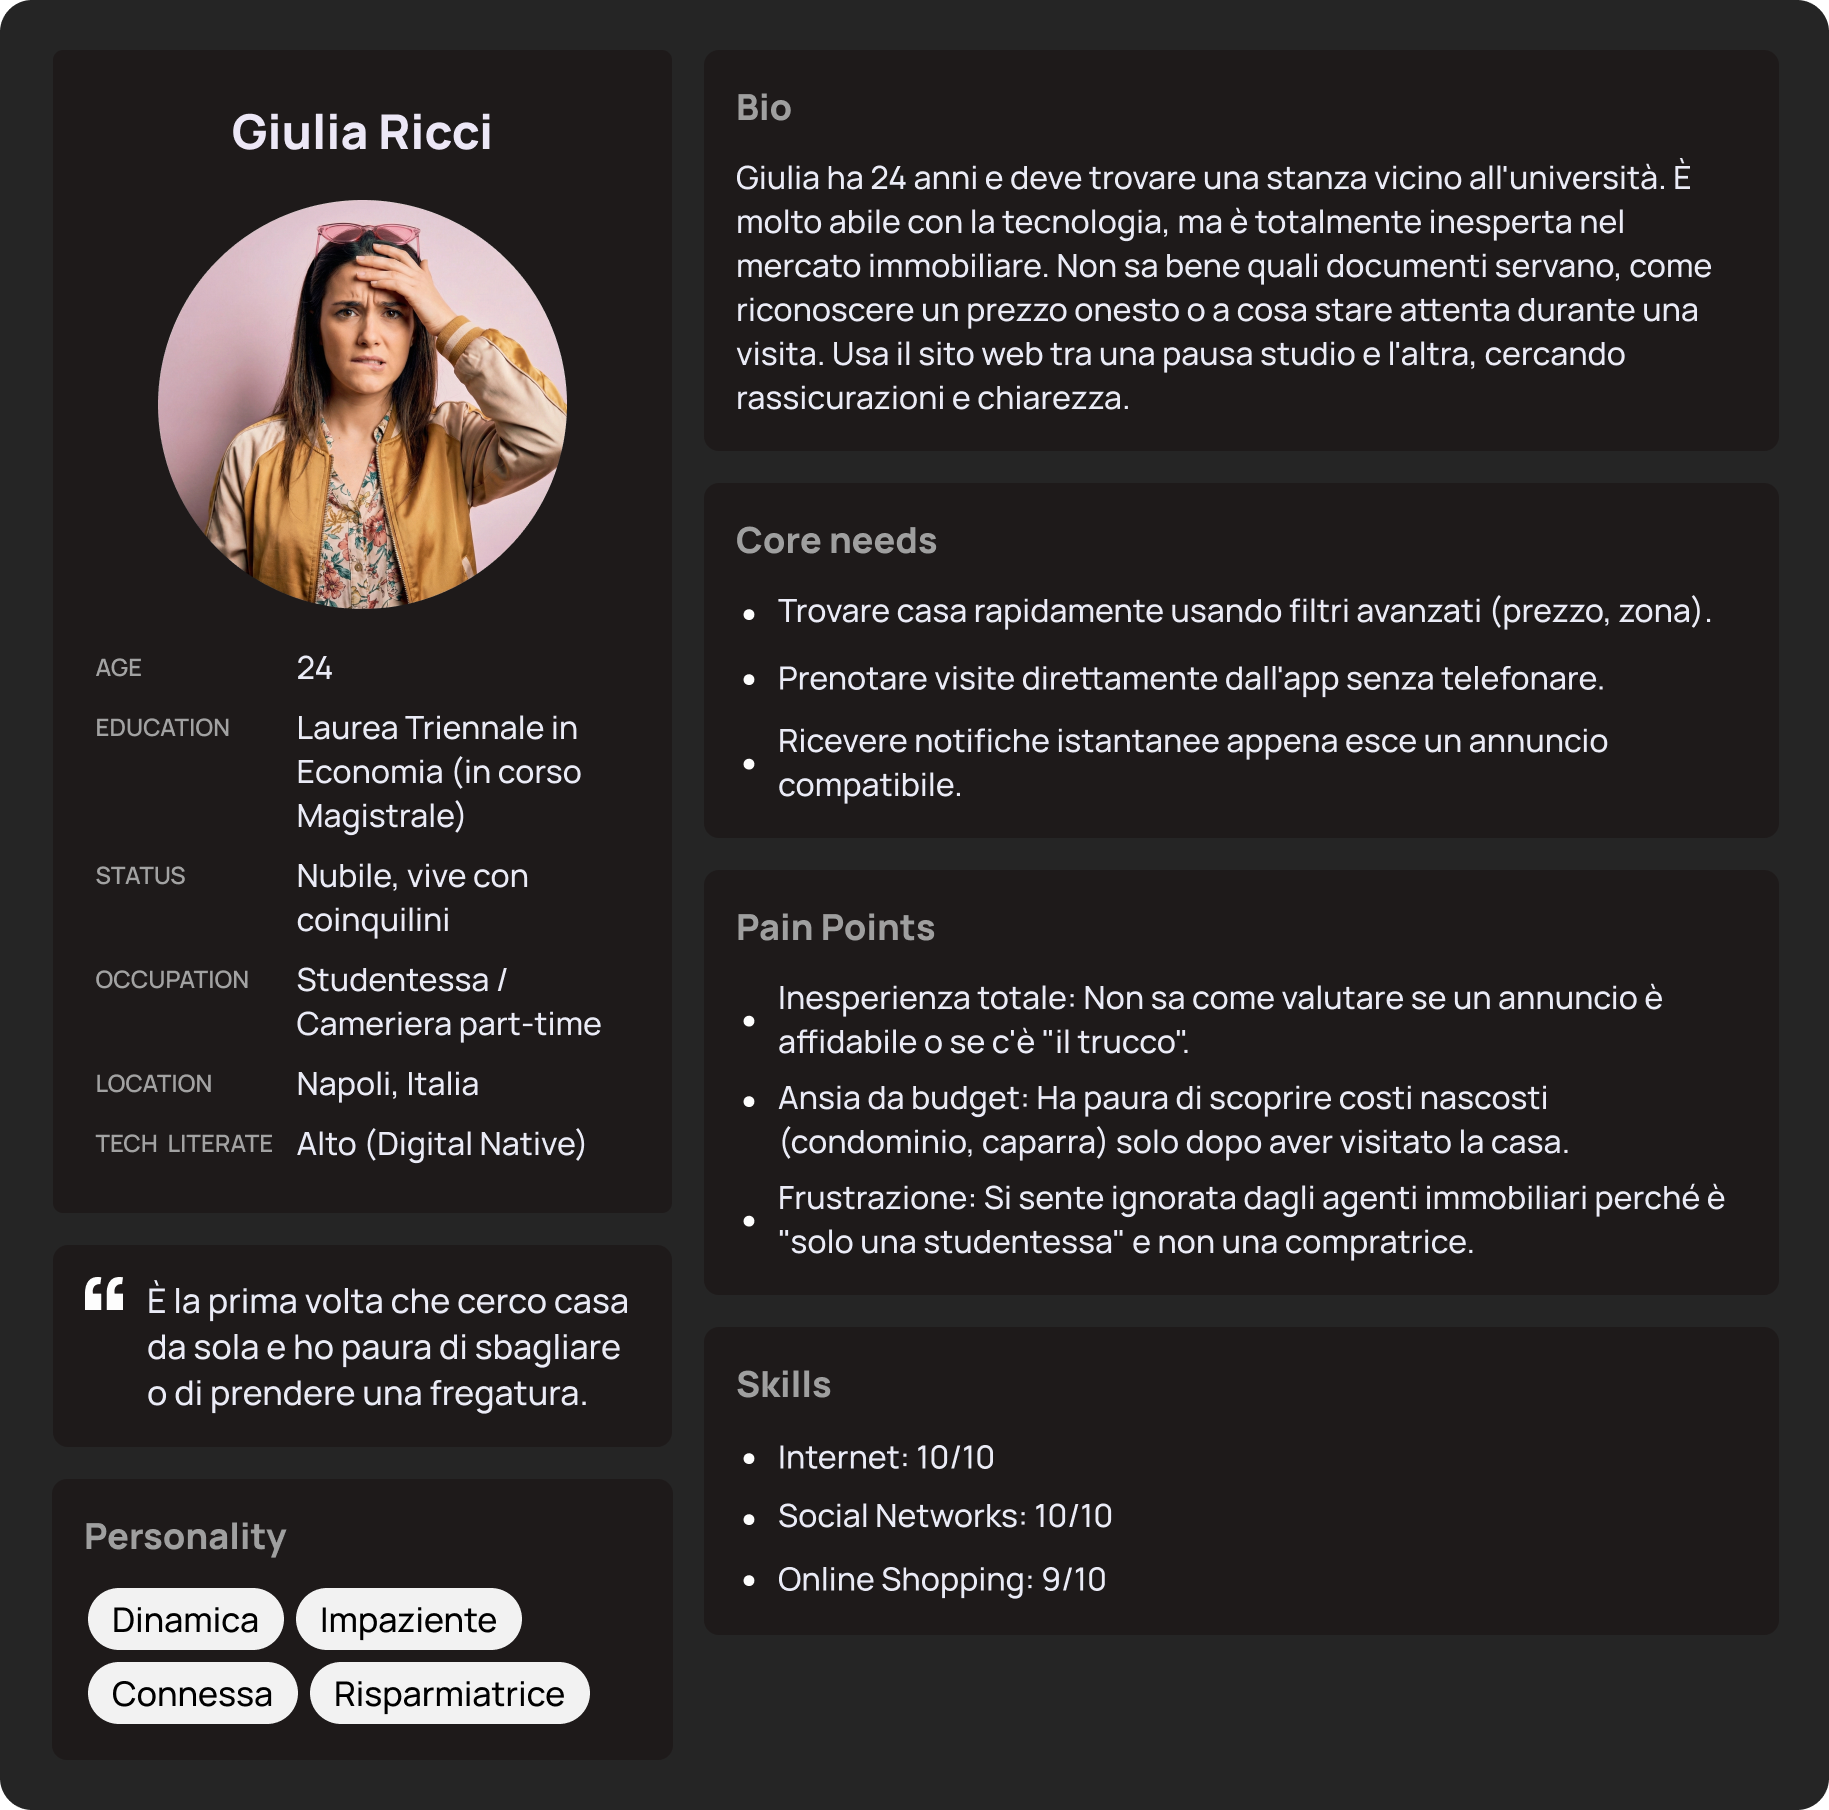
\includegraphics[width=0.8\textwidth]{images/Giulia.png}
     \caption{Personas Studentessa Universitaria - Giulia Ricci}
     \label{fig:P1}
 \end{figure}

   \subsection{Antonio Bianchi  - Utente Poco Esperto di Tecnologia}

  \begin{figure}[H]
     \centering
     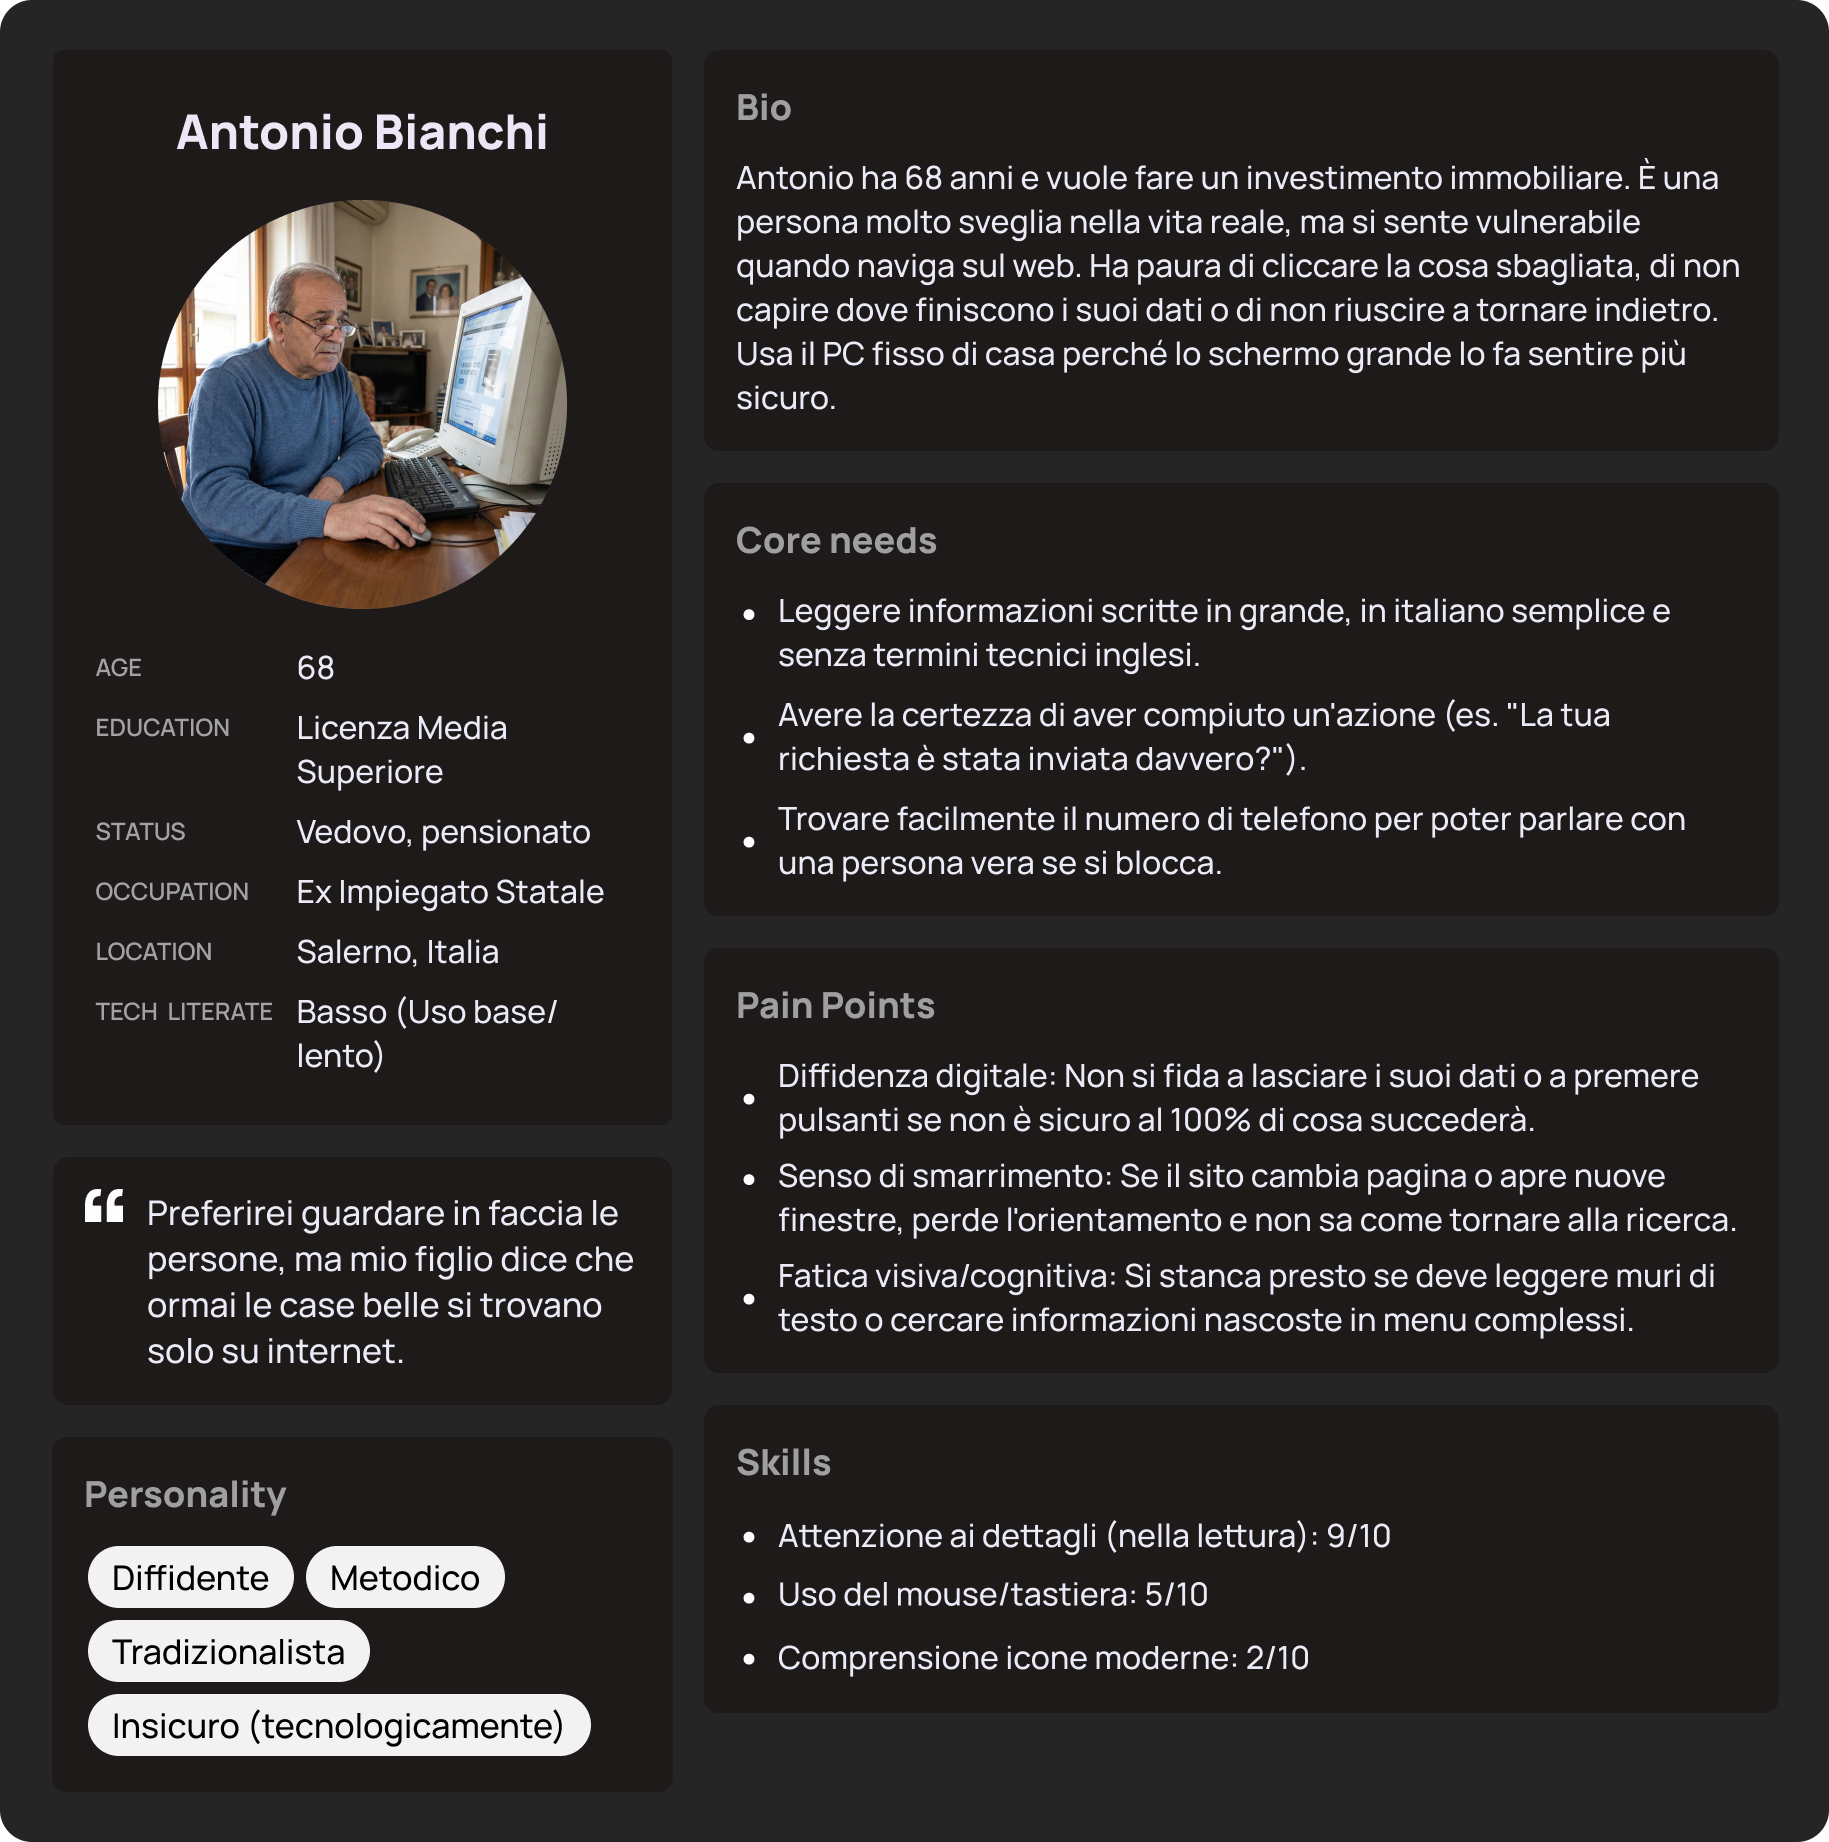
\includegraphics[width=0.8\textwidth]{images/Antonio.png}
     \caption{Personas Utente Poco Esperto di Tecnologia - Antonio Bianchi}
     \label{fig:P2}
 \end{figure}
 
  \subsection{Marco Esposito  - Agente Immobiliare}

  \begin{figure}[H]
     \centering
     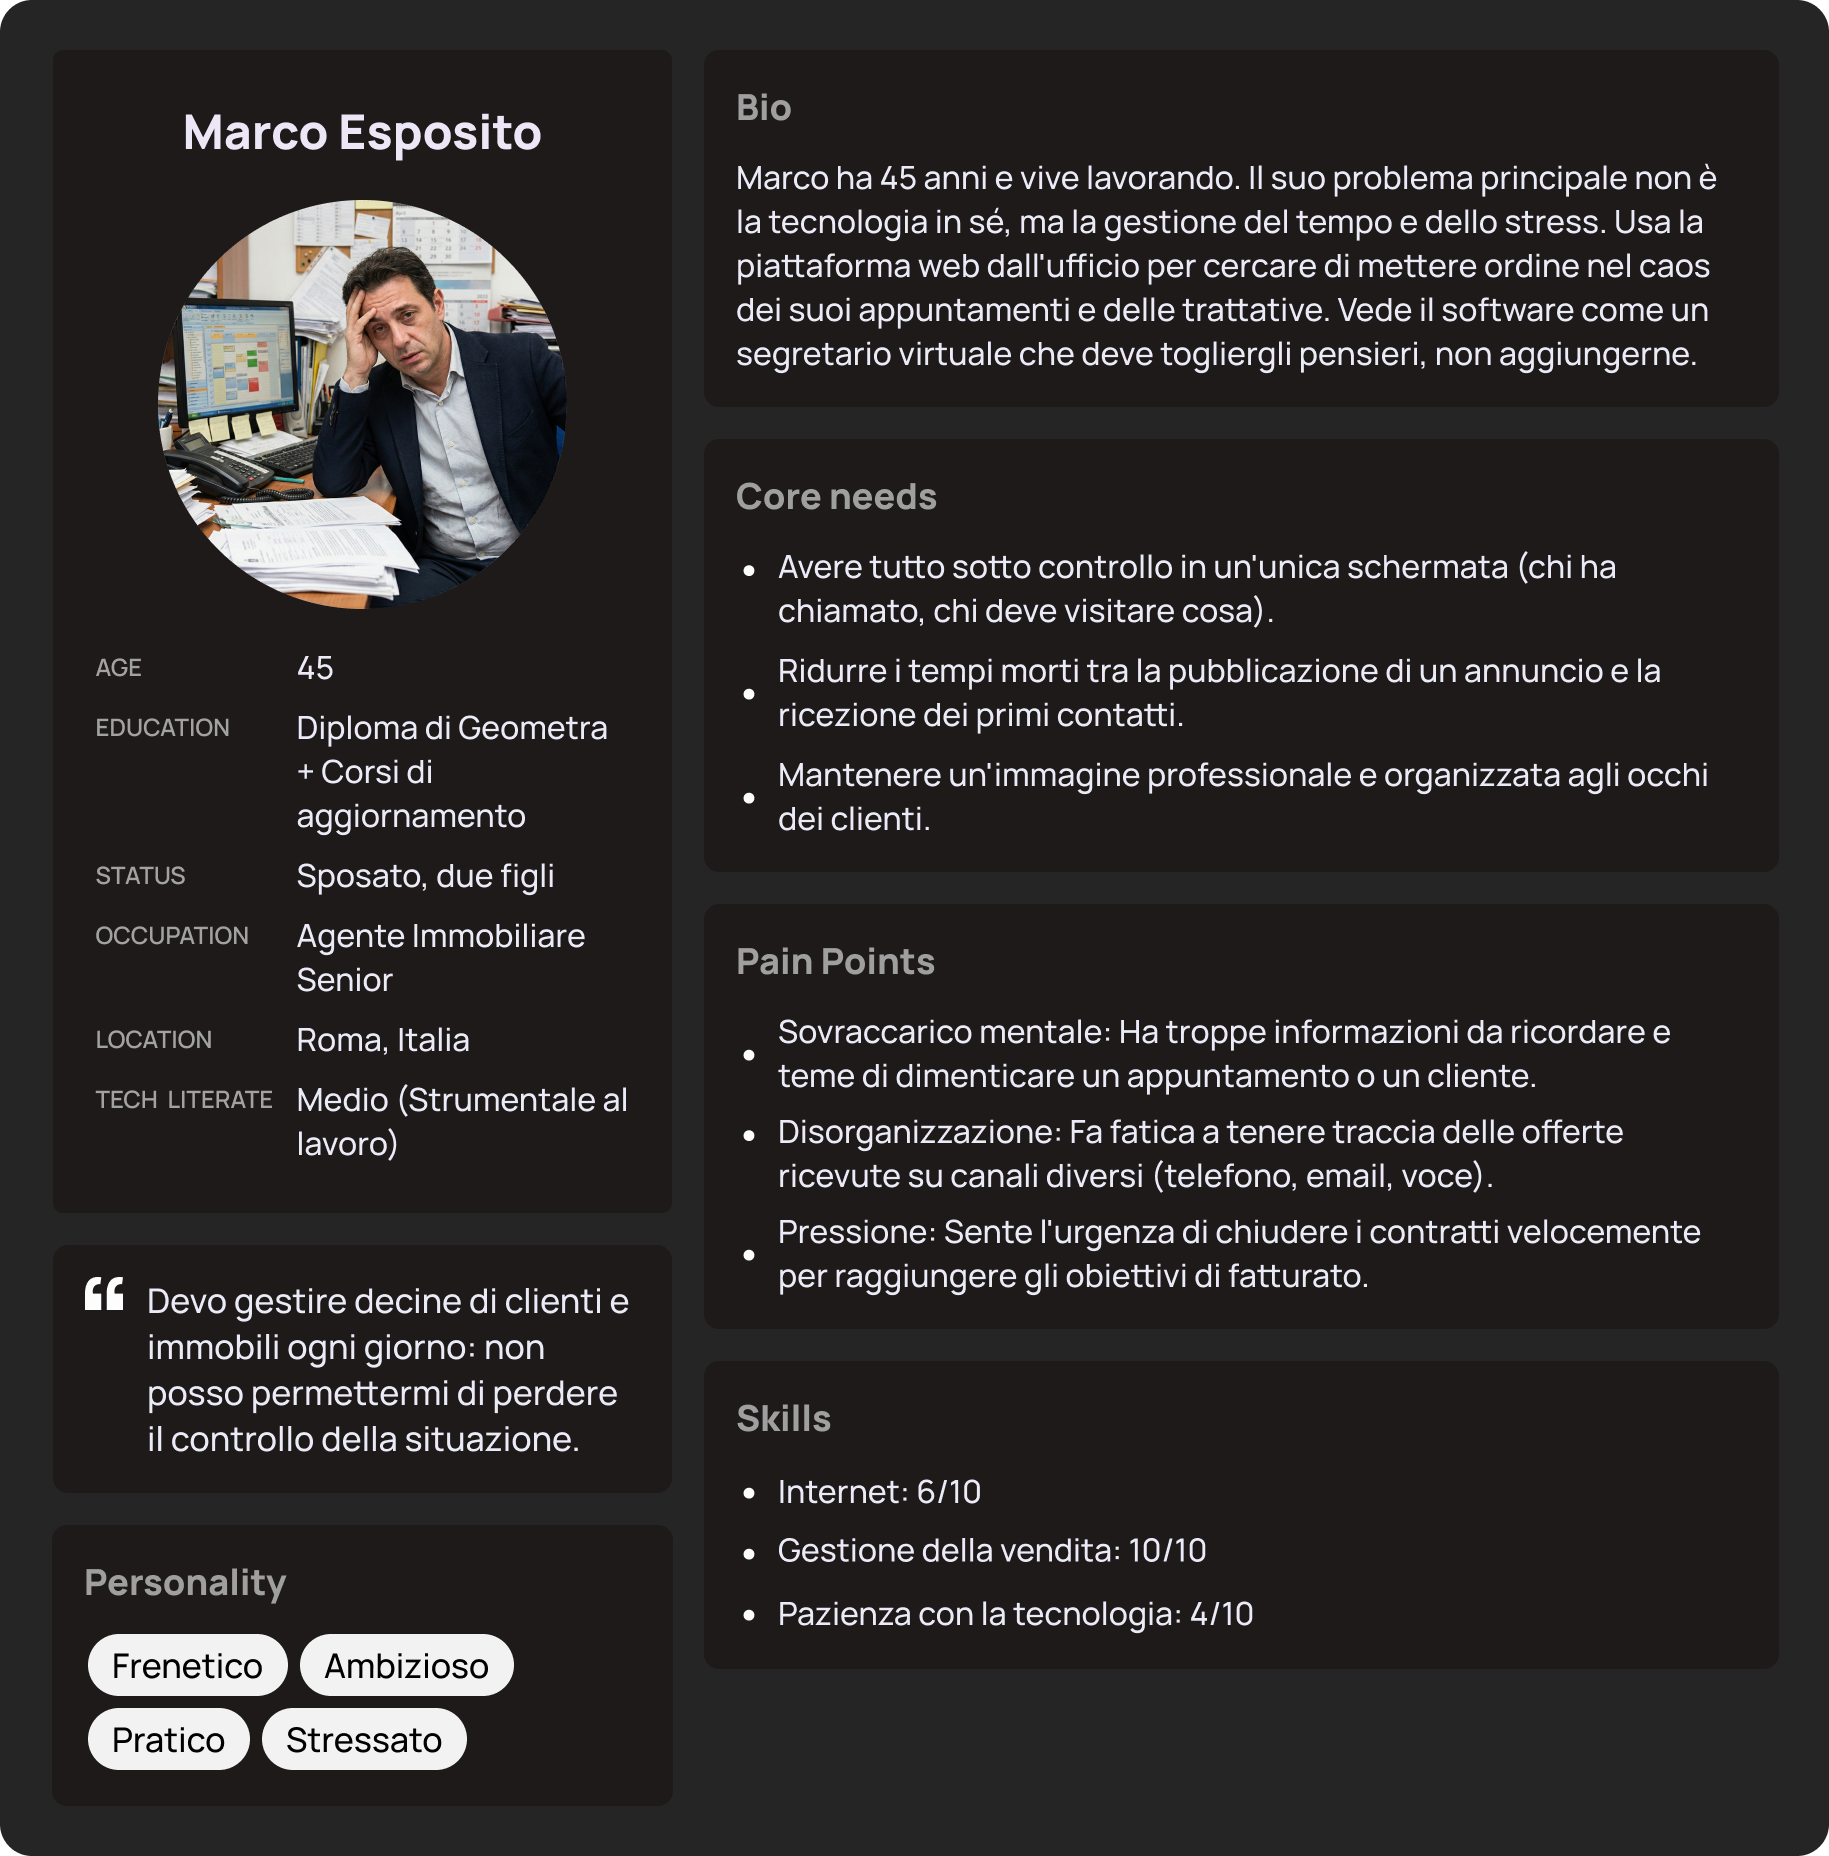
\includegraphics[width=0.8\textwidth]{images/Marco.png}
     \caption{Personas Agente Immobiliare - Marco Esposito}
     \label{fig:P3}
 \end{figure}

   \subsection{Roberto De Luca  - Manager di Agenzia Immobiliare}

  \begin{figure}[H]
     \centering
     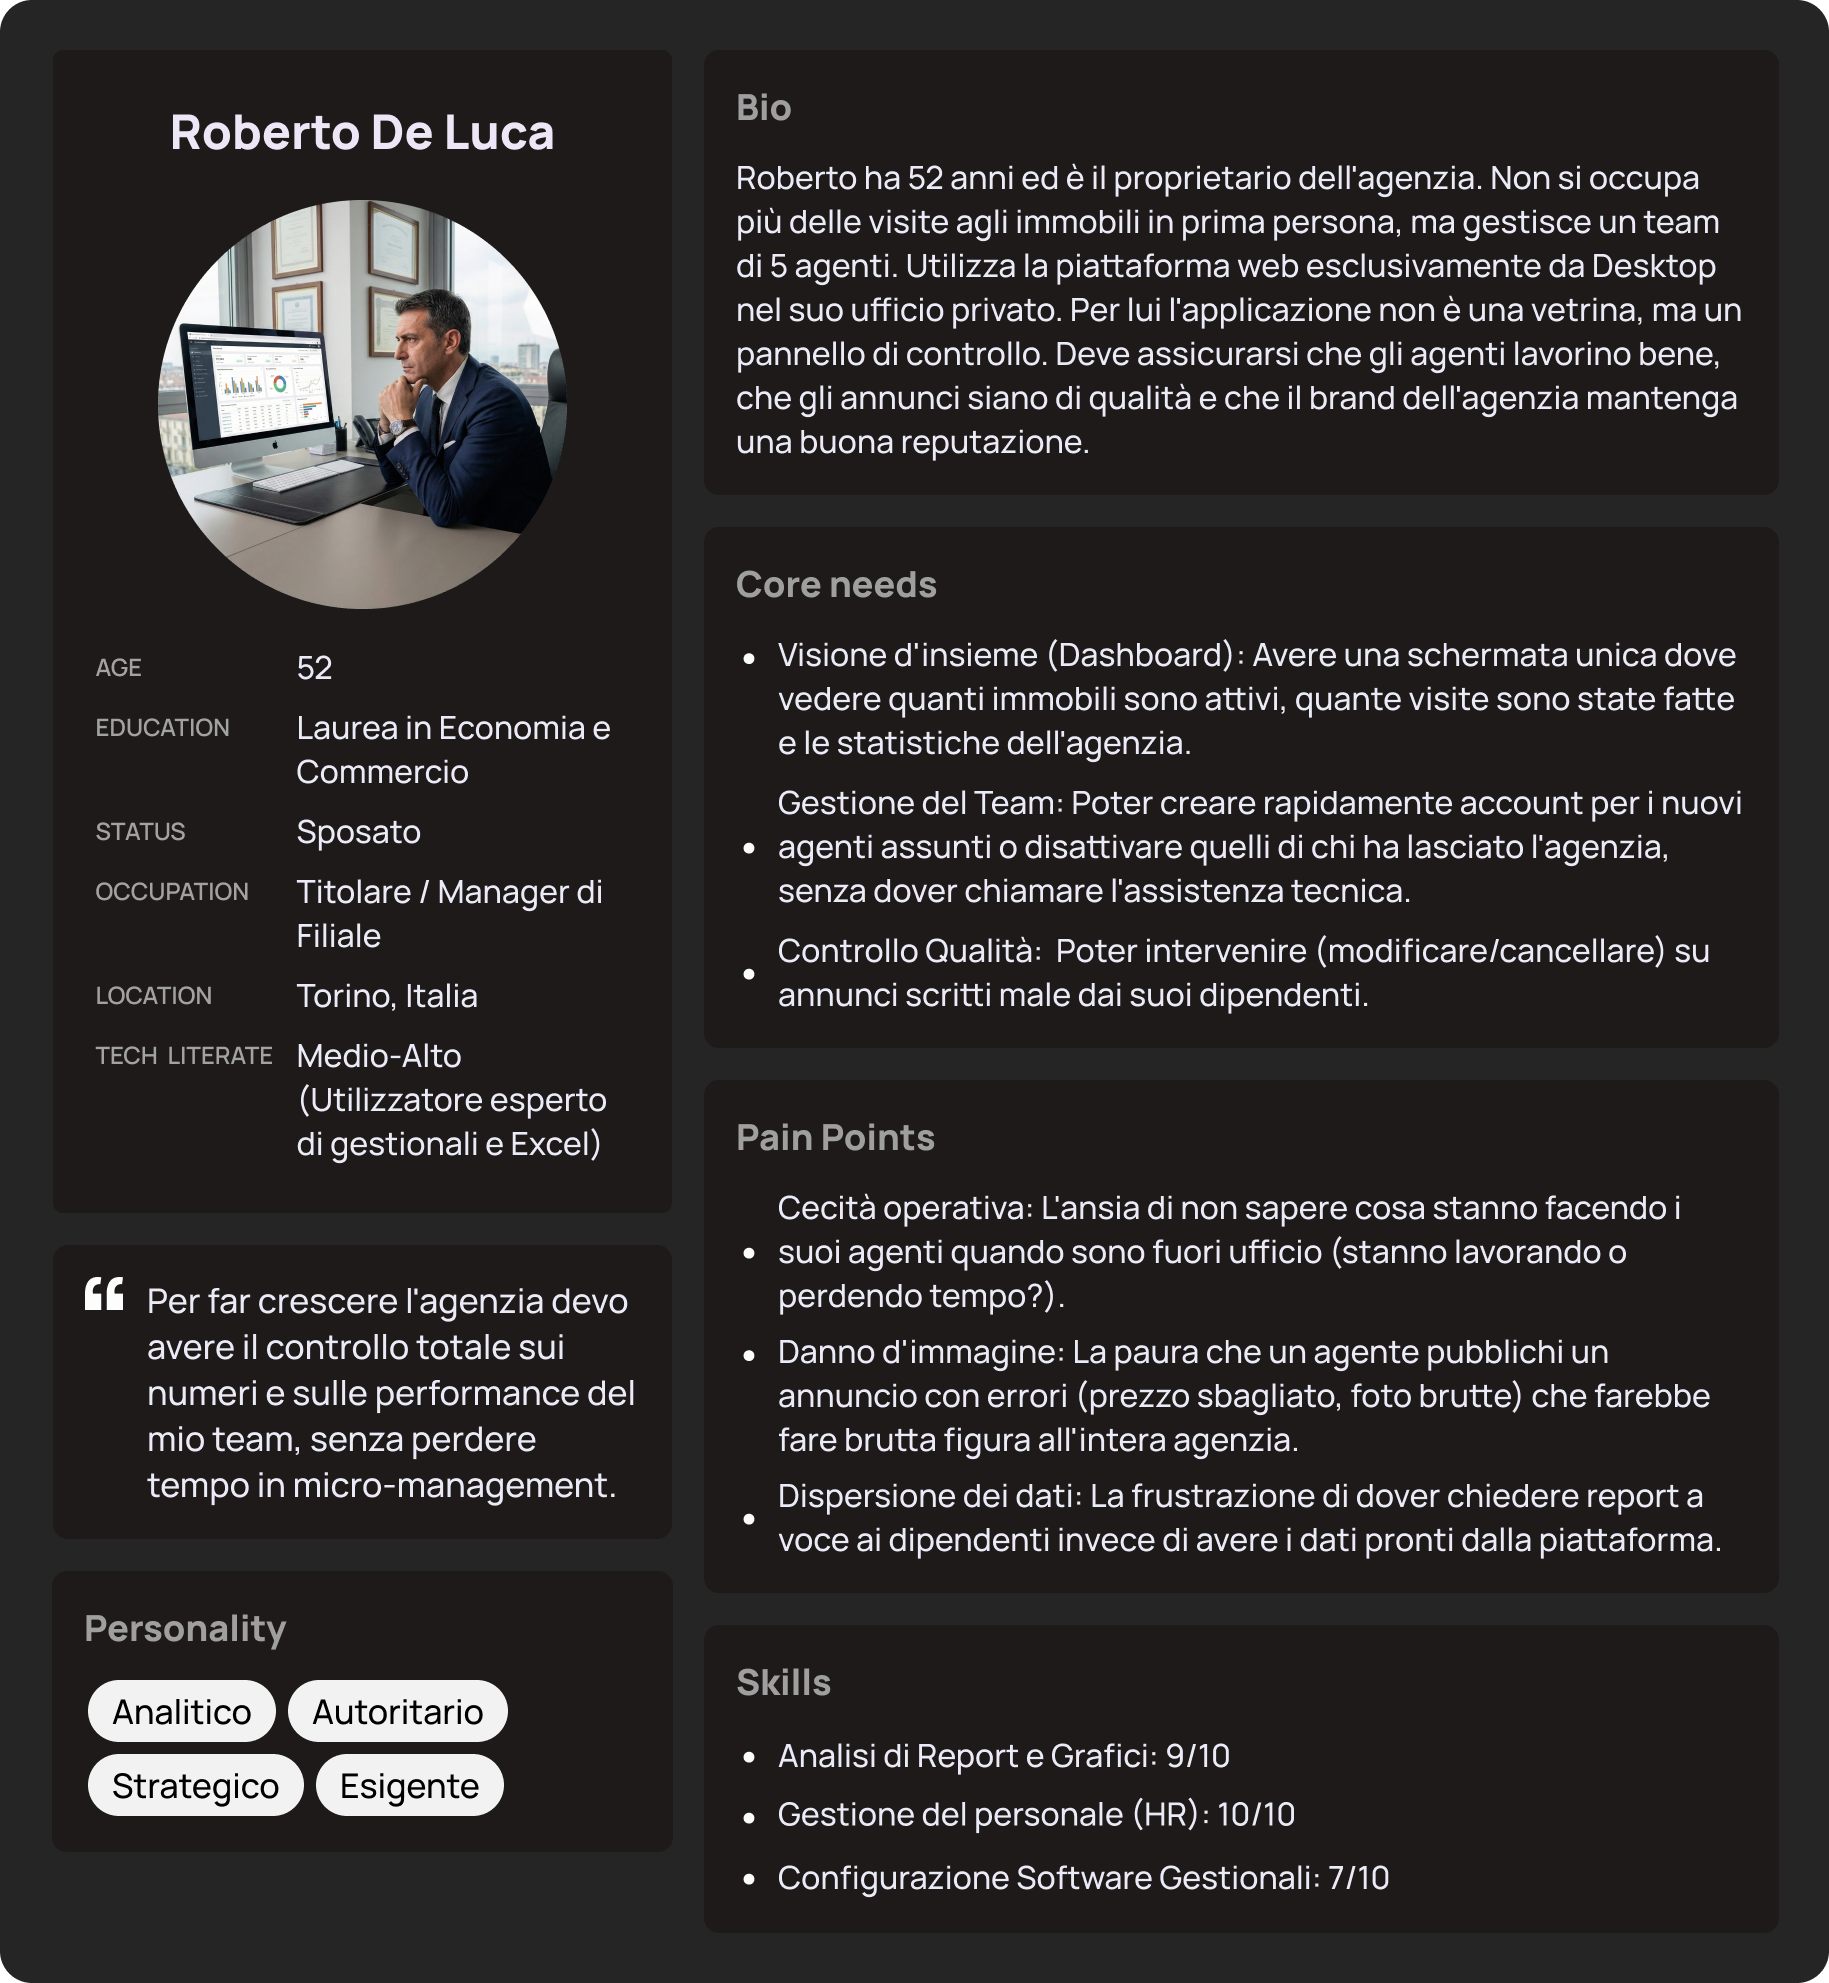
\includegraphics[width=0.8\textwidth]{images/Roberto.png}
     \caption{Personas Manager di Agenzia Immobiliare - Roberto De Luca}
     \label{fig:P4}
 \end{figure}
 
